\chapter{}\label{chap3}
\addtocontents{toc}{\bigskip}
\addtocontents{toc}{\protect\contentsline{chapter}{\protect \centerline{Chapter \numberline{\thechapter}}}{}}  
\addtocontents{toc}{\medskip}

\section*{Visitors, associates and others}
\addtocontents{toc}{\protect\contentsline{section}{Visitors, associates and others}{\thepage}}

\lhead[{\it\fontsize{9pt}{9pt}\selectfont\thepage}]{\it{\fontsize{9pt}{11pt}\selectfont Visitors, associates and others}}

\index{Raman Research Institute|(}
Raman loved\index{Raman, Chandrasekhara Venkata!Traits/Interests} to talk about his Institute, his research and
about himself. When he was in a good mood, you could not meet
a person more inspiring and lovable than him. In the event he
was in a bad mood, it was prudent to stay away from him. Princes
and politicians, statesmen and scientists, students and teachers
regularly visited the Institute to see Raman and talk to him.
He gave them an enthusiastic welcome and took them round the
museums, lecture theatres and on to the verandas or the portico
for a view of the distant vista and the surrounding gardens.
He talked to them about his current activities and sometimes took
them into the laboratory for a first-hand experience of the
phenomenon he was studying.

To  some he showed his memorabilia, the medals, the
honorary doctoral gowns and the precious gifts he had received.
Among these the Nobel Diploma and the Nobel Medal figured
prominently. The Diploma was of exquisite calligraphy in a
tastefully decorated format. The heavy gold medal with Alfred
Nobel in relief on it was something everyone wanted to touch
and feel. The honorary doctoral gown of the University of Paris\index{University of Paris}
was a very impressive and colourful piece of dress with cap to
match. Raman would have looked majestic when he walked down
the aisle, along with the academics of the University of Paris,
to receive the honorary doctorate conferred on him. He once told
me that he had earned only a Masters degree in physics; all the
doctorates were {\em honoris causa}. Raman kept all his memorabilia
locked in steel almirahs in his downstairs room and the keys to
these secured in a steel safe.

He had an elaborate system of locks and keys to the
laboratories and steel cabinets. In the beginning, only he would
open the safe and give the keys to the museums, or to any other
room to be opened. As time went on, he gained confidence in
me and Padmanabhan\index{Padmanabhan, J.} and allowed us access to the heavy steel
safe. Each bunch of keys to the rooms and cabinets had its allotted
place in the safe and we were instructed to strictly adhere to the
arrangement. It was a sight to see Raman walking with a bunch
of keys and opening the rooms himself for visitors. We received
a duplicate set of keys to our laboratory rooms. In respect of
keys, he treated me with special consideration and trusted me with
the master key to the safe, whenever he went out of town for any
length of time. The reason for all the safety and precaution was
understandable in view of the precious nature of things he kept.

In the early days of the Institute, Raman was quite generous
in admitting visitors and taking them round himself. Sometimes
he would ask me or Padmanabhan to show visitors around. Later,
he found visitors a great impediment to his work and for the peace
and quiet he needed. So he began to discourage visitors, except
the very important ones. He even installed a notice board at the
entrance to the Institute, ``No Admission to Visitors''.

Among the eminent scientists who visited Raman, the
following come to mind: J.D. Bernal,\index{Bernal, J.D.} H.J. Bhabha,\index{Bhabha, H.J.} E.C. Bullard,\index{Bullard, E.C.}
S. Chandrasekhar,\index{Chandrasekhar, S.} C.G. Darwin,\index{Darwin, C.G.} P.A.M. Dirac,\index{Dirac, P.A.M.} J.B.S. Haldane,\index{Haldane, J.B.S.}
Linus Pauling,\index{Pauling, Linus} C.F. Powell,\index{Powell, C.F.} Norbert Wiener\index{Wiener, Norbert} and G. Wentzel.\index{Wentzel, G.} The annual Indian Science Congress,
 usually held every January, used to sponsor the visits of foreign scientists for its meetings.
Most of these scientists would come to Bangalore, for it was not
only an important centre for science but India's most distinguished
scientist also lived and worked there. In addition, Bangalore is
a lovely city with many attractions for the visitors and is the
gateway to Mysore --- one of the most colourful cities in India,
famed for its Maharajahas' palace, the Krishnaraja Sagar
reservoir and for the nearby Bandipur game sanctuary. The Indian
Institute of Science\index{Indian Institute of Science} and Raman Research Institute would be on
the itinerary of every visiting scientist.

The Russian scientific delegation used to be the largest of
all the scientist groups in those days and was quite visible at every
Science Congress. These delegations would have someone at the
level of an Academician as the leader and a number of younger
scientists accompanying him. The Russian scientists without
exception came to visit Raman. At one time, Raman was out of
town and we had to take care of one such Russian delegation.
Academician N. V. Belov,\index{Belov, N. V.} a well-known Russian crystallographer,
was the leader. There were also a number of young scientists with
him. They were so disappointed with Raman's absence that they
had their itinerary rearranged so that they could visit the Institute
again, a week or so later, when Raman was back.

Apart from these invitees to the Science Congress, other
eminent scientists from abroad came as special invitees of the
Government of India and Bangalore was always on their itinerary.
Therefore Raman had visitors the year round. He generally
showed great enthusiasm in receiving them and taking them
around. He lectured to them on his latest findings. At other times
he tried to convince them of his views. One of his favourite topics
was his lattice dynamical theory; he was severely critical of the
viewpoint of Max Born\index{Born, Max} on this subject. Although Raman had
invited Max Born to Bangalore in the Thirties and had deep regard
for Born as a physicist, he was totally opposed to Born on the
theory of lattice dynamics. Some of the visits of prominent
scientists to the Raman Institute during the period between 1950
and 1960 are described below and in the following pages.
\index{Raman Research Institute|)}

\medskip
\heading{J.D. Bernal}
\index{Bernal, J.D.}
\smallskip

\noindent
Bernal was one of the earliest distinguished visitors to the
Raman Institute. I think it was the 1950 Science Congress for
which he was invited and he came to Bangalore after participating
in it. Raman took Bernal round the Institute with great enthusiasm
and showed him some of the experiments that we were doing at
the time using sunlight. Bernal was a brilliant X-ray physicist,
crystallographer, crystal physicist and crystal chemist, all rolled
in one. He had a keen mind and a very scholarly look.

Bernal was, at the time, a Professor at Birbeck College,
London.\index{Birbeck College, London} He knew of Raman's work on lattice dynamics and the
raging controversy between Raman and Max Born. He was even
more conversant with the controversy over diamond in which
Raman and Kathleen Lonsdale\index{Lonsdale, Kathleen} were involved. This related to the
X-ray diffraction effects in diamond (the so-called extra
reflections). Whenever Raman talked about these things, Bernal
smiled enigmatically, but his remarks were measured and he did
not endorse the explanations that Raman offered or his views.

One afternoon, Raman offered to take him round Bangalore
in his Willys sedan. Raman's younger son, Radhakrishnan,\index{Radhakrishnan, V.} and
I also went with them. After visiting Cubbon Park and Lalbagh,
we ended up at the Bull Temple in Basavangudi. One of the most
impressive sights in this temple is the gigantic stone bull at the
entrance. Raman explained to Bernal the role of the bull in a
Siva temple. Then we went near the {\em sanctum sanctorum} and there
was this Trident --- the famous weapon of Siva --- just outside
the inner chamber. Bernal asked about the significance of the
Trident and its purpose and Raman explained it to him. It was
a very pleasant outing, which we all enjoyed very much.

\medskip
\heading{H.J. Bhabha}
\index{Bhabha, H.J.|(}
\smallskip

\noindent
Bhabha was one of the most eminent physicists of India.
He was mainly responsible for founding India's Nuclear Energy
programme. He was born in 1909 in Bombay and was connected
to that well-known industrial family, the Tatas. He initially
enrolled in Gonville and Caius College in Cambridge\index{Gonville and Caius College, Cambridge} in 1927 to
study mechanical engineering, but switched to theoretical physics
and took a B.A. degree in 1930. Paul Dirac\index{Dirac, P.A.M.} was, apparently, one
of his tutors. Bhabha received his Ph.D. in 1935 for his research
on cosmic ray-produced electron showers at the Cavendish
Laboratory in Cambridge.\index{Cavendish Laboratory, Cambridge} He stayed on in Cambridge until 1939.

During this period he spent time with Fermi's group in Rome,
Pauli's group in Zurich and Niels Bohr's\index{Bohr, Niels} Institute in Copenhagen.
Bhabha's work with Heitler in 1937, on cosmic ray showers
produced by muons, and other work in the field earned him a
lasting reputation in theoretical physics. He returned to India in
1939 at the outbreak of World War II for a vacation and,
fortunately for India, could not return to Cambridge.

He joined the Indian Institute of Science\index{Indian Institute of Science} as Professor of
cosmic ray physics. Raman was at the time heading the Physics
Department and encouraged Bhabha. With Raman's support, and
through his own Tata connections, Bhabha was able to create
a new Institute particularly devoted to research on cosmic rays
and nuclear physics. The Tata Institute of Fundamental Research\index{Tata Institute of Fundamental Research}
was founded in Bangalore in June 1945 with Bhabha as its
Director. It later moved to Bombay. When the Indian Atomic
Energy Commission\index{Indian Atomic Energy Commission} was established in 1948, Bhabha was made
its Chairman. The Commission conducted most of its early
research and development work at the Tata Institute of Fundamental Research.

Bhabha was a frequent visitor to Bangalore in the early
Fifties, coming there to supervise the balloon flight experiments
carried out by the cosmic ray research unit of the Tata Institute
of Fundamental Research. Bhabha was actively involved in cosmic
ray studies in those days and was regarded as a front-ranking
scientist in the field. Raman and Bhabha were on very friendly
terms and, during his Bangalore trips, Bhabha used to come to
the Raman Research Institute to see Raman. On one occasion,
he even brought his mother to the Institute.

Bhabha was very interested in art and himself painted.
He drew a line sketch of Raman in 1949, a reasonably successful
portrayal.

In the mid-Fifties Bhabha got deeply involved in India's
atomic energy development project. He did an excellent job
organising the Agency, the laboratories and the atomic energy
programmes. He received considerable encouragement from
Government and had direct access to Prime Minister Nehru.\index{Nehru, Jawaharlal}
Consequently, his power and prestige increased enormously and
he became the most influential scientific administrator in India.
He became the first Chairman of India's Atomic Energy
Commission and held the post until his premature death in an
airplane crash in the Swiss Alps on January 24, 1966.

Bhabha simultaneously held three important positions in
India, namely, the chairmanship of the A.E.C., Secretary to the
Government in the Department of Atomic Energy and Director
of the Tata Institute of Fundamental Research.\index{Tata Institute of Fundamental Research} Bhabha was a
superb organiser and was able to function efficiently in all three
capacities. However, he gave up active science himself to emerge
as the most powerful scientific administrator in the country.

Raman hated big organisations and felt a big bureaucracy
only wasted money. He began to feel uncomfortable with Bha\-bha
and gradually the two drifted apart. Bha\-bha never visited Raman
after 1954 and I think this upset Raman very much. He used to
open up the latest research volumes and ask visitors, ``Do you
find the name of Bhabha anywhere in the scientific literature
nowadays? He has quit Science''.\index{Bhabha, H.J.|)}

\medskip
\heading{E.C. Bullard}
\index{Bullard, E.C.}
\smallskip

\noindent
Bullard was Director of the National Physical Laboratory\index{National Physical Laboratory, England}
in England at the time he visited India and called on Raman in
Bangalore. Bullard immensely enjoyed Raman's conducted tour
of the Institute. On this occasion, Raman showed him all his
personal memorabilia, including the Nobel Medal, the Nobel
Diploma, the Hughes Medal of the Royal Society, the Franklin
Medal and the Metucci Medal. Several colourful doctoral gowns
worn by Raman during the award of Honorary Doctorates were
also shown to Bullard. Bullard was particularly interested in
Raman's relationship with Rutherford.\index{Rutherford} Raman had a great regard
for Rutherford and spoke highly of him and his majestic
personality. Rutherford strongly endorsed Raman's candidacy
for the Nobel Prize and supported him on several occasions.
Raman and Rutherford had many similarities. Both were very
powerful, domineering personalities, and led very active schools
of physics in their respective countries.

\medskip
\heading{S. Chandrasekhar}
\vskip .1cm
\index{Chandrasekhar, S.|(}

\noindent
Subrahmanyan Chandrasekhar, the distinguished Professor
of the University of Chicago, is Raman's nephew. He won the
Nobel Prize for Physics in 1982 for contributions he had made
to astrophysics almost fifty years earlier.

Chandrasekhar was born in 1910 in Lahore and took his B.Sc.
Hons. degree in physics in 1930 from Presidency College,\index{Presidency College} Madras,
the same college that Raman had gone to some 25 years earlier.
When Chandrasekhar was finishing his B.Sc. Hons.degree,
Raman had just then won the Nobel Prize for Physics. Therefore
the influence of Raman's life on young Chandrasekhar must have
been strong. The bright young physicist set the highest goals for
himself and left for Cambridge to pursue higher studies in physics.

He turned to theoretical astrophysics, inspired by a book
by\break Eddington\index{Eddington} that he had received as a prize. Even as a student
at Presidency College, Madras, he had given thought to
fundamental astrophysical problems and some of the important
ideas concerning the fate of a dying star crystallised in his mind
on the voyage to England. While in Cambridge, he came into
contact with the celebrated astrophysicist, Eddington himself, and
discussed astrophysics on a day-to-day basis with him.
Chandrasekhar's work in Cambridge, led to a rigorous solution
to the puzzle concerning the fate of a star which had gone through
its nuclear burning cycles and begun cooling. On January 11,
1935, at a meeting of the Royal Astronomical Society in London\index{Royal Astronomical Society, London}
he presented a paper on the subject, in the presence of\break Eddington.
Immediately after Chandrasekhar's presentation, Eddington got
up and vehemently criticised Chandrasekhar's theory.

According to the ideas prevailing then, a cooling star would
undergo gravitational collapse, and become a dense ball called
a white dwarf. Chandrasekhar studied this collapse when the
gravitational force was sufficient to overcome the counteracting
electronic pressure of the compressed dense gas arising from the
operation of the Pauli exclusion principle. Chandrasekhar proved
conclusively that a star with a mass greater than 1.4 solar mass
would collapse into dense matter in which the electrons have
velocities close to that of light --- a state called relativistic
degeneracy. This would cause the star to go on collapsing beyond
the white dwarf stage, losing energy through radiation until it
becomes so dense that light is trapped and the star vanishes.
Such a situation is now known as black holes, but at that time
examples of white dwarfs, neutron stars --- a dense star consisting
of only neutrons --- or black holes were unknown to observational
astronomy.

Chandrasekhar's theory had far-reaching consequences, and
modern astronomy and astrophysics have vindicated his
conclusions. Eddington, however, did not like to believe in
such an ignominious fate for a stellar object and, hence, opposed
Chandrasekhar's brilliant and fundamental contribution. The
latter felt undermined by this and was deeply disappointed with
Eddington's attitude.

In 1936, Chandrasekhar migrated to Chicago to accept a
professorship at the University of Chicago\index{University of Chicago} and has remained there
ever since. He changed his subject to radiative transfer, stellar
structure and magnetohydrodynamics, but in later years worked
on black holes again. He is now interested in general relativity.
In each of these areas he has made monumental contributions.
Finally, due recognition for his original contribution came in 1982
when he was awarded the Nobel Prize for physics, which he shared
with William A. Fowler\index{Fowler W.A.} of the California Institute of Technology.\index{California Institute of Technology}
Chandrasekhar's books on magnetohydrodynamics and black
holes are classics.

Chandrasekhar visited Bangalore in 1951. This, I believe,
was his first visit to India after he moved to Chicago in 1937.
He was then near 40. The Chandrasekhars stayed with Raman.
Raman's remark on meeting Chandrasekhar is noteworthy.
Commenting on the fact that Chandrasekhar had not been back
in a long time, he said, ``You are visiting India like Halley's
comet''. Raman was quick-witted and would say the most
unexpected things.

When Chandrasekhar visited the Raman Institute,\index{Raman Research Institute} we had
no electricity, but a lot of light-scattering experiments were going
on with sunlight. We were studying the diffusion of light in
moonstone at the time. Raman had shown that the geometry of
the observed halo and its dimensions contained information about
the size and shape of the particles responsible for the optical
heterogenity and we had worked out that these could be estimated
using a simple optical diffraction theory. Raman demonstrated
the effect to Chandrasekhar and the latter was quite impressed
by the optical phenomena and the explanation offered by Raman.
He suggested that Mie's theory of scattering could be applied to
the situation. However, Raman's simple approach and the
explanation he advanced was an intuitive jump over any
mathematical theory. Chandrasekhar was shown some of the
other experiments that were going on at the time, using sunlight.
One of them was the luminescence of diamond, which always
impressed visitors.

Raman was very proud of Chandrasekhar's achievements
and proposed him for the Nobel Prize as early as the Fifties.
During that visit to Bangalore, Chandrasekhar gave a lecture on
``The Polarisation of the Sunlit Sky'' at the Indian Institute of
Science before a huge audience. Raman, who sat in the front row,
appreciated the masterly presentation very much.
\index{Chandrasekhar, S.|)}

\medskip
\heading{C.G. Darwin}
\index{Darwin, C.G.}
\smallskip

\noindent
Darwin, a famous X-ray physicist from England, came to
Bangalore to meet Raman. A visit to the Raman Institute\index{Raman Research Institute} and
a dinner at Raman's home later in the evening had been planned.
Darwin came to the Institute in the morning and Raman, as was
customary, took him round the laboratories and the museums.
Then he talked about his lattice dynamical theory with a view
to gaining approval of his ideas. He gave a well-prepared lecture
for 45 minutes. Darwin listened to it and then responded, ``I don't
agree with your ideas''.

Raman was infuriated. Very upset, he said, ``I wasted my
time. You are all prejudiced. I should have known that this
business of trying to convince a British physicist is as bad as trying
to unbend a dog's tail''. Darwin was no younger than Raman
and he was taken aback by these remarks. Suddenly the warmth
and enthusiasm that Raman had shown Darwin evaporated.
When taking leave of Raman later that morning, Darwin actually
doubted whether the dinner engagement was still on. He asked
Raman, ``Are we meeting for dinner?'' Raman replied,
``Yes, yes --- we are having dinner at my house in the evening''.
But Raman continued to feel that the whole British School of
Physicists was influenced strongly by Max Born\index{Born, Max} and, hence,
opposed to his views.

\medskip
\heading{P.A.M. Dirac}
\index{Dirac, P.A.M.|(}
\smallskip

\noindent
Dirac's visit to the Raman Research Institute in 1954 was
a very pleasant affair, with Raman very happy throughout. In
fact, Raman had planned a 3-day visit to Bangalore for Dirac
and had filled it with so many engagements that he left very little time for 
Dirac even to visit the Indian Institute of Science.\index{Indian Institute of Science}
However, these plans got altered when Dirac arrived as the guest
of the I.I.Sc. Nevertheless, he came to the Raman Institute and
spent quite some time with Raman. The next day, Raman took
him in his car to visit his country home and a nearby water
reservoir called Thippagondanahalli.

When Dirac came to the Institute, Raman took him round
enthusiastically and showed him everything that was to be seen
there. He gave a talk on his lattice dynamics at the lecture theatre;
this was attended by a few others as well. After the 45-minute
presentation, Raman wanted to know Dirac's opinion about
his theory. Dirac began to respond rather slowly. He started
saying that ``What you presented appears reasonable'', but
before anything further was said Raman took Dirac's hand and
warmly shook it, saying, ``I know you will see my point of view.
You are one of the greatest physicists for whom I have a great
regard''. Dirac could not, and did not, make any further
comments. Raman was certainly under the delusion that Dirac
agreed with him.\index{Dirac, P.A.M.|)}

\medskip
\heading{J.B.S. Haldane}
\index{Haldane, J.B.S.|(}
\smallskip

\noindent
Haldane was an eminent British biologist who fell in love
with India and settled there in his later years. After he settled
in India, he even wore dhotis in the Bengali fashion and thus
identified himself with the country totally. He made Bhubanes\-war
in Orissa his home and carried on research in biology, agriculture
and statistics applied to biology.

Haldane was one of those rare individuals who had a broad
interest in Science. He knew mathematics, physics, chemistry and
biology. He was a tall, hefty figure and had a commanding
personality.

His trip to the Raman Institute was memorable. He gave
a talk at the Indian Institute of Science in the morning and
was to visit the Raman Institute after the talk. He refused the
car that was arranged to take him to the Raman Institute and
walked the one mile at a brisk pace. A lot of admirers walked
with him; it was like a {\em Padayatra} (pilgrimage on foot) to the
Raman Institute.

Raman received him at the portico and conducted him
thro\-ugh the Institute. His first remark was, ``Prof. Haldane, why
did they make you walk? I would have sent my car''. To this
Haldane replied that he preferred to walk and enjoyed the exercise
very much. Raman took Haldane round his museum and proudly
showed him his bird and mollusc collection to impress him that
his interest in biology was a match for Haldane's.
\index{Haldane, J.B.S.|)}

\medskip
\heading{Mark Oliphant}
\index{Oliphant, Mark}
\smallskip

\noindent
Sir Mark Oliphant, a distinguished Australian nuclear
physicist who had worked under Rutherford,\index{Rutherford} came to India in
1956 to deliver the Rutherford Memorial lecture. Alladi Ramakrishnan,\index{Ramakrishnan, Alladi} the Director of the Mathematical Sciences Institute,\index{Mathematical Sciences Institute}
Madras, had invited Oliphant to deliver the lecture in Madras.
Oliphant had a written lecture and was planning to deliver the
same lecture in both Madras and Bangalore. It was arranged that
the lecture in Bangalore would be chaired by Raman.

Ramakrishnan narrates how a reporter from the Madras
daily, {\em The Hindu}, interviewed Oliphant and planned to publish
the gist of the lecture. But as the reporter left, Oliphant
inadvertently handed him the entire transcript of the lecture.
The next morning, {\em The Hindu} carried the lecture verbatim over
four columns, as a tribute to the great scientist Ernest Rutherford.
Raman read the speech in {\em The Hindu} and promptly called
Oliphant, who had just arrived in Bangalore and was staying at
the West End hotel, to say that he had read the lecture given in
Madras and that he had enjoyed it very much. Oliphant, it seems,
was quite embarrassed about it, since he could not give the same
speech again, especially with Raman in the chair. Fortunately
he had another version, which he delivered and thereby avoided
any amusing comments from Raman.

The lecture by Oliphant was given at the Sir Puttannachetty
Hall in Bangalore before a distinguished audience of scientists,
students and general public. I was in the audience and heard
Raman speak in glorious terms about the lecture and about
Rutherford.

\smallskip
\medskip
\heading{Linus Pauling}
\index{Pauling, Linus}
\medskip

\noindent
Pauling visited Bangalore in 1954 and came to see Raman. Raman took him round with great enthusiasm and showed him his exquisite collection of gems, minerals and crystals. He also gave a short talk on his lattice dynamics and waited for Pauling's comments. Pauling, however, did not commit himself and merely said, ``I will have to think about it more deeply''.

Pauling had been awarded the Nobel Prize for chemistry shortly before he visited India. In the upper portico of the Raman Institute\index{Raman Research Institute} quite a few scientists had assembled on the day of Pauling's visit and someone remarked that Pauling had been awarded the Nobel Prize for chemistry. Raman promptly said, ``I elected him to the honorary fellowship of the Indian Academy of Sciences\index{Indian Academy of Sciences} years ago, knowing his worth. The Nobel Committee has recognised his greatness only now''. Raman was evidently quite happy with himself for the remark and Pauling responded with a smile.

Raman had taken a little more time than was allotted for the visit. Pai, who was the Registrar of the Indian Institute of Science\index{Indian Institute of Science} and who had been accompanying Pauling, made some rude remarks to Raman about his delaying his visitor. Pauling had to rush to the Indian Institute of Science to deliver a lecture on ``Sickle Cell Anemia and its Molecular Biological Basis''. It was strange that Raman let the remarks pass. We all felt that a nonscientist like the Registrar had no business to talk to Raman in that fashion.

\newpage
\heading{C.F. Powell}
\index{Powell, C.F.}
\smallskip

\noindent
Powell was a distinguished cosmic ray physicist from Bristol who came to India in 1956 at the invitation of H.J. Bhabha.\index{Bhabha, H.J.} Powell pioneered the use of the photographic emulsion technique for recording cosmic ray encounters as tracks in the plate, and discovered several new particles from the cosmic ray-produ\-ced tracks on photographic plates. He won the Nobel Prize for Physics in 1950. M.G.K. Menon,\index{Menon, M.G.K.} a well-known Indian scientist turned scientific administrator, worked under Powell and participated in some of the experiments conducted in the early Fifties.

\vskip .06cm

Powell visited Bangalore during his trip and called on Raman. The latter wanted to trace the origin of the use of the photographic emulsion technique in recording cosmic ray encounters and I remember him going to the Indian Institute of Science Library to investigate. After much searching Raman found that Blau\index{Blau} and Wambacher\index{Wambacher} had in 1907 discovered the photographic emulsion technique whose use Powell had pioneered. Raman triumphantly talked about his findings to Powell and the latter was amazed by Raman's curiosity and thoroughness.

\vskip .06cm

Those were great days for cosmic ray physics and cosmic ray physicists. Powell gave a scintillating talk and Raman enjoyed the lecture very much.

\bigskip
\noindent
\heading{S. Bhagavantam}
\index{Bhagavantam, S.}
\smallskip

\noindent
Bhagavantam joined Raman as a research scholar in Calcutta at the comparatively young age of 18 and Raman intuitively recognised the great potential and precocity of the young scientist. Bhagavantam commenced his research career with investigations on the optical and magnetic anisotropy in aromatic and aliphatic series of compounds and established the relationship between the magnetic behaviour of organic crystals and their molecular form and crystal structure. Soon after the discovery of the Raman Effect in 1928, Bhagavantam took up the study of the Raman spectra of gases. His pioneering work on the effect of pressure on the Raman spectra of gases helped in elucidating the influence of intermolecular collisions and viscosity on the rotational structure of the Raman bands in gases.

In 1932, Bhagavantam joined the Andhra University,\index{Andhra University} Waltair, where he remained for sixteen years, becoming successively Professor, Head of the Department of Physics and then Principal of the University Colleges. During this period, besides continuing his investigations on the Raman Effect, he established an active school of experimental research in ultrasonics and developed new techniques for the measurement of the elastic constants of crystals. His two books published during this period, namely {\em Scattering of Light and Raman Effect} and {\em Theory of Groups and its Applications to Physical Problems},
are still among the best books that any research worker can find on the respective topics. The second book, with Venkatarayudu\index{Venkatarayudu} as co-author, is perhaps one of the most important contributions to the understanding of the Raman spectra of crystals. Through the use of group theory, Bhagavantam and Venkatarayudu established the role of crystal symmetry in splitting the degenerate vibrational levels of molecules and molecular groups when they go into crystals to occupy positions of symmetry.

Bhagavantam\index{Bhagavantam, S.} possessed the rare combination of scientific eminence and administrative ability and consequently held a variety of important positions during his career. He was chosen as the first scientific liaison officer of independent India in the U.K. On his return, he went to Hyderabad as Professor of Physics
and started an active research school at the Osmania University.\index{Osmania University} Later, he became the Vice-Chancellor of Osmania University. During this period, he initiated work in cosmic ray research, studies on high polymers and solid state physics, and published his third valuable book, {\em Crystal Symmetry} and {\em Physical
Properties}. He also took steps to rejuvenate astronomical studies and research in Hyderabad.

From 1957 to 1962, he served as Director of the Indian Institute of Science,\index{Indian Institute of Science} Bangalore. Later at the invitation of the then Defense Minister, V.K. Krishna Menon,\index{Krishna Menon, V.K.} with whom he had become friends during his London days, Bhagavantam became scientific adviser to the Ministry for Defense, Government of India. He also held many other important professional positions and his career was one of laudable achievements.

Bhagavantam remained a loyal friend of Raman throughout and the latter had a special affection for Bhagavantam. He used to treat Bhagavantam very warmly and the latter, in turn, had a deep regard for Raman. I have seen them together on innumerable occasions, engrossed in discussion. Bhagavantam never failed to attend the Executive Council meetings of the Indian Academy of Sciences,\index{Indian Academy of Sciences} of which I was a member, by virtue of my position as the Treasurer of the Academy, from 1956 to 1961. Bhagavantam hosted several annual meetings of the Academy while he was in Hyderabad and at Andhra University. In fact, the first Academy meeting I went to was in December 1950; it was hosted by Osmania University where Bhagavantam was the Director and Professor at the Physical Research Laboratory.

Raman used to enjoy Bhagavantam's lectures, which were notable for their precision, clarity and thoroughness. Bhagavantam died in February 1989 at the age of 80. When I visited him in the first week of December 1988, he recalled his Calcutta days and talked about Raman.

\medskip
\heading{K.S. Krishnan}
\index{Krishnan, K.S.|(}
\smallskip

\noindent
K.S. Krishnan joined Raman in Calcutta as a research scho\-lar in 1923. Krishnan was a very capable experimenter and worked on several problems in optics and magnetic and electric double refraction in anisotropic molecules. Raman and Krishnan discussed, in a series of papers, the magnetic double-refraction in liquids and the electric double refraction in relation to the polarity and optical anisotropy of molecules.

Krishnan's outstanding record of research won for him first the M.Sc. and, later, the D.Sc. degree of the Madras University.\index{University of Madras} He assisted Raman in the light-scattering experiments at those very crucial stages which led to the discovery of the Raman Effect. The first few publications relating to the discovery, and the subsequent detailed papers, were published jointly by Raman and Krishnan. His collaboration with Raman continued up to 1930 when he accepted the Readership in Physics at Dacca University.\index{Dacca University}

Krishnan continued in Dacca, with a band of dedicated scholars and post-graduate workers, his remarkable series of studies on the magnetic susceptibility of many organic and inorganic compounds. He returned to the Indian Association for Cultivation of Science,\index{The Indian Association for Cultivation of Science} as the first Mahendralal Sircar Professor in 1933, when Raman left Calcutta to take up the Directorship of the Indian Institute of Science\index{Indian Institute of Science} in Bangalore. A few years later, Krishnan was elected as a Fellow of the Royal Society, London. He moved to Allahabad University\index{Allahabad University} as Professor of Physics in 1942. There, he became attracted to theoretical physics, influenced
by A.B. Bhatia,\index{Bhatia, A.B.} a brilliant mathematician, who had joined him as a research student. Krishnan continued in Allahabad until 1947, carrying on an excellent research tradition.

The British Government conferred upon him the knighthood in recognition of his outstanding scientific work in Allahabad. Soon after, he accepted the invitation to become the first Director of the National Physical Laboratory in New Delhi,\index{National Physical Laboratory, New Delhi} a position he held until his death in 1961. Krishnan received many honours and distinctions during his lifetime.

Krishnan had wide interests and was a noted scholar in Tamil. He was a very good speaker with a subtle sense of humour and was an excellent conversationalist. It appears that Prime Minister Nehru\index{Nehru, Jawaharlal} liked Krishnan very much and enjoyed a chat with him whenever he had some free time.

I first saw Raman and Krishnan together in Delhi in 1951, at the time the Indian Academy of Sciences' annual session was held there. Raman used to be the chairman of a committee called the Physical Research Committee instituted by the Council of Scientific and Industrial Research\index{Council of Scientific and Industrial Research} and Krishnan was a member of this committee. Consequently, Krishnan used to come to Bangalore periodically for these meetings and Raman and Krishnan were on very friendly terms. But after 1953, their relationship deteriorated and was completely destroyed.

\newpage

It is difficult to fathom how this happened. Many versions were current at the time. In 1953, which was the Silver Jubilee year of the discovery of the Raman Effect,\index{Raman, Chandrasekhara Venkata!Raman Effect} feeble voices were heard whispering that Krishnan had played a significant role in the discovery. These reached Raman's ears and, lacking the patience to verify the veracity of these stories and their source, he jumped to the conclusion that Krishnan entertained such ideas. He felt humiliated and let down, and began to regard Krishnan unfavourably. Friends and well-wishers of both were helpless in this drama. Raman's feelings were so strong, they caused much anxiety in the minds of many. This was a very unpleasant episode in the life of Raman and Krishnan.

\vskip .1cm

Unfortunately such views still find expression. For instance, Sankar Chakraborty\index{Chakraborty, Sankar} states in the {\em Calcutta Municipal Gazette}\index{Calcutta Municipal Gazette@\textit{Calcutta Municipal Gazette}} of No\-vem\-ber 2, 1988, ``In the discovery of the Raman Effect, K.S. Krishnan played a very significant role. Many have felt that K.S. Krishnan should have been acknowledged as the co-discoverer of the effect now bearing Raman's name exclusively''. You go into the history of the discovery of the Raman Effect, it is very clear that the light-scattering programme was initiated and led by Raman in Calcutta, soon after he returned from his first European trip in 1921. During the years 1921 to 1928, Raman had several collaborators working with him on the subject, and they included K.R. Ramanathan,\index{Ramanathan, K.R.} K. Seshagiri Rao, S. Venkateswaran,\index{Venkateswaran, S.} K.S. Krishnan and a few others. Of this team, Krishnan undoubtedly was involved very much in the final phase of the discovery and there was therefore a very close and intense collaboration between Raman and Krishnan. In such a collaboration, only the two participants can speak about their roles and it would be impossible for outsiders to assign credit. Further, the Nobel Committee goes thoroughly into these matters and they seem to have had no difficulty in identifying Raman's leading role in the light-scattering programme in Calcutta, which culminated in the discovery of the Effect which his scientific peers in the field at that time named as the `Raman Effect'. It is to be noted that the Nobel citation for Raman reads ``for his investigations on the scattering of light and the discovery of the effect known after him''. It is not just for the final discovery alone.

Raman has generously acknowledged the assistance of Krishnan in the discovery, as well as the contributions of his other collaborators. Further, most of the papers relating to the new discovery bear the name of Raman and Krishnan. More importantly, Krishnan had never claimed in public that his contributions to the discovery were suppressed. An unbiased chronicler would have no difficulty in identifying the leading role played by Raman in the light-scattering work and would probably also conclude that Raman would have discovered the Effect without the assistance of anyone. However, it must be said that it was one of the most effective collaborations in the history of science; it certainly helped to bring the subject to a quick culmination at a time when the time element was very important. Otherwise, full credit for the discovery would probably have been lost, in the light of the events that followed, namely the independent observation of the light-scattering effect by the Russian scientists Landsberg\index{Landsberg} and Mandel'shtam,\index{Mandel'shtam} who were behind only by a few months.

To me it all sounds so sad and utterly futile to make an issue of this monumental contribution to Science by one of the most illustrious sons of India.
\index{Krishnan, K.S.|)}

\medskip
\heading{K.R. Ramanathan}
\smallskip

\index{Ramanathan, K.R.|(}

\noindent
Ramanathan was one of the earliest associates of Raman. He was born in Kalpathi, Palghat, on February 28, 1893, about five years after Raman. He had his early education in Victoria College,\index{Victoria College} Palghat, and took his Bachelor's degree in physics from the Presidency College,\index{Presidency College} Madras. Then he joined Maharajaha's College in Trivandrum and served there as a lecturer for seven years. He joined Raman in Calcutta as a University of Madras\index{University of Madras} research scholar towards the end of 1921 and collaborated with him in the studies of the molecular scattering of light and X-ray diffraction in liquids, gases and mixtures. Within a period of one year he had published ten papers and was awarded the D.Sc. degree of the University of Madras for his thesis based on this work. He then accepted a teaching appointment in Rangoon in 1922, but continued to visit Raman's laboratory in Calcutta during the vacations.

During these periods, he conducted intensive examination of the molecular diffraction of light by water. Using sunlight and complementary filters, Ramanathan detected a weak residual light, which was dismissed as ``weak fluorescence'' due to impurities. However, in later years, Raman pursued this very ``weak fluorescence'' systematically and this pursuit led to the discovery of the Raman Effect in 1928.

In 1925, Ramanathan joined the India Meteorological Department\index{India Meteorological Department|(} and retired as its Deputy Director General in 1948. After his retirement he took up the Directorship of the Physical Research Laboratory\index{Physical Research Laboratory} at Ahmedabad and set up, for the first time in India, a group to investigate the physics of the upper
atmosphere. He retired from the Directorship in 1966, but continued to work as Emeritus Professor.

He also helped Dr.~Vikram Sarabhai\index{Sarabhai, Vikram} organise space physics research in its initial stages in India. Ramanathan was held in high regard by the Sarabhai family and was truly a friend, philosopher and guide to the young Sarabhai. He passed away in Ahmedabad on December 31, 1984, at the age of 91.

Raman had great affection and regard for Ramanathan. Since the latter was only five years younger, Raman treated him as a colleague. Ramanathan served the Meteorological Department with distinction for 23 years and there he established high scientific standards. He brought physics into meteorology and
built up the department with outstanding physicists, who were mostly Raman's students. In those days, the only two avocations open to young physicists in India were either teaching or as meteorologists in the Meteorological Department. Raman chose Ramanathan to high offices in the Indian Academy of Sciences.\index{Indian Academy of Sciences}
At the annual meetings of the Indian Academy of Sciences, Raman loved to hear Ramanathan expound on subjects connected with the upper atmosphere and atmospheric physics and enlisted him for public lectures at these meetings.

I have seen at close quarters the genuine mutual affection that existed between Raman and Ramanathan. To Ramana\-than, Raman was a great hero and his beloved professor. To Raman, Ramanathan was a symbol of devotion and loyalty. Love and affection dominated their relationship. Only once was this relationship disturbed for a brief period. That was in 1953, when the Silver Jubilee of the discovery of the Raman Effect was being celebrated.

It was a minor incident in Bombay that strained this intimate relationship. Ramanathan inadvertently made a remark, during a public meeting connected with the celebration in Bombay, that Raman used the mercury arc by accident to discover the Raman Effect; that since it was a rainy day Raman had decided to use the mercury arc. Within a few days, a visitor from Bombay to the Raman Institute\index{Raman Research Institute} mentioned this to Raman, without realising the impact it would have on him. Raman was infuriated beyond control and totally lost his bearings. That was Raman's character when he was hurt. We did not understand at first why he was so upset, but the story soon unfolded.

Raman sent a telegram to Ramanathan asking him to come and explain to him why he had made such a statement. Ramanathan took the next plane and arrived in Bangalore to face Raman. Raman and Ramanathan were closeted in the former's office for a long time and then the two came out. Ramanathan issued a statement to the Press retracting what he had said and profusely apologised for the mistake he had made. After that, the relationship between Raman and Ramanathan returned to normalcy and the unpleasant episode was soon forgotten.
\index{India Meteorological Department|)}
\index{Ramanathan, K.R.|)}

\medskip
\heading{L.A. Ramdas}
\index{Ramdas, L.A.}
\smallskip

\noindent
Ramdas joined Raman in Calcutta, in 1923, as a Palit Research Scho\-lar and conducted experiments on the scattering of light by mercury and other pure liquid surfaces. Besides this, he investigated the optical properties of monomolecular films spread on water surfaces and the movement of surface-active substances like camphor on water. After obtaining his Ph.D. in Calcutta under Raman, he joined the \hbox{India} Meteorological Service in 1926, but continued to visit the \hbox{Indian} Association for Cultivation of Science\index{The Indian Association for Cultivation of Science} in Calcutta during his vacations to actively work with Raman. It was Ramdas who named the light-scattering effect discovered by Raman as the ``Raman Effect''.

His work in the Meteorological Department was mainly involved with research problems connected with meteorology. He established and developed the new Division of Agricultural Meteorology in Pune, which specialised in the physics of the earth-atmosphere boundary layers. He pioneered research in this area. After retirement, Ramdas continued his researches in physics and atmospheric physics at the National Physical Laboratory in New Delhi.\index{National Physical Laboratory, New Delhi}

Ramdas, who had a deep respect and admiration for Raman, was a frequent visitor to the Raman Research Institute\index{Raman Research Institute} in Bangalore. Another attraction for him in Bangalore was his son, A.K. Ramdas,\index{Ramdas, A.K.} who worked as a research scholar under Raman.

Ramdas had a fine sense of humour and it was a delight for us to listen to his stories about Raman's Calcutta days and about his own experiences with people. Ramdas wrote two very fine articles on Raman in the {\em Indian Journal of Physics Education} in 1971 and 1973. In these articles, he has given an authentic and accurate picture of Raman's Calcutta days, for he was a part of those days. He has thrown much light on this period of Raman's life and his description of Raman as a teacher is perhaps the only one of its kind available. I have used quite a bit of material from these two articles in this work, for which I am indebted to him very much. Ramdas had planned a third article. Unfortunately, this did not materialise and much rich material of the Calcutta days has been lost.

\medskip
\heading{Vikram Sarabhai}
\index{Sarabhai, Vikram}
\smallskip

\noindent
Vikram Sarabhai admired Raman and had the highest regard and respect for him. In fact, he spent some time as a disciple under Raman, at the start of his research career. He was a frequent visitor to Bangalore.

The Sarabhai family are wealthy mill owners in Ahmedabad and the whole family was very attached to Raman, who had, on \hbox{several} occasions, been their guest at their home in Ahmedabad. They helped him in his efforts to collect money for building the Raman Research Institute, donating generously, themselves, and influencing their\break friends to contribute substantially to the cause.

Vikram Sarabhai was the only one in the family who took to Science. He started his scientific career as a cosmic ray researcher and became a well-known contributor in the field. Subsequently, he moved on to organising the Space Science effort in India. This has now grown into a huge, Government-sponsored research organisation. After Bhabha's\index{Bhabha, H.J.} death in the aircrash, the Chairmanship of India's Atomic Energy Commission fell on Sarabhai's shoulders. Thus, he had the awesome responsibility, at one and the same time, of two large Government Departments, each employing thousands of scientists and engineers. Sarabhai had such fine human qualities and a superb managerial capacity that he was liked by everyone who came into contact with him, enabling him to smoothly run both organisations.

Raman was very fond of Vikram Sarabhai and encouraged him in his research. He also gave him several opportunities to conduct symposia on cosmic ray research during the annual meetings of the Indian Academy of Sciences.\index{Indian Academy of Sciences} I distinctly remember the 1953 annual meeting held in Ahmedabad when Sarabhai and his group presented talk after talk at a symposium on cosmic ray studies in India.

Fifteen years later (1968), the Academy met in Ahmedabad to celebrate the 80th birthday of Raman. This was a happy occasion in which many Fellows participated and paid their tributes to the doyen of Indian Science. Sarabhai actively participated in this meeting and was, in fact, its principal architect. Despite his very busy schedule, he was present throughout the conference.

One afternoon, Sarabhai\index{Sarabhai, Vikram} and Raman were seated and chatting on the lawns adjacent to the Physical Research Laboratories where the meetings were being held. I had just joined them when Raman asked Sarabhai how he was able to manage three jobs, shuttling between Delhi, Ahmedabad, Bombay and Trivandrum and overseeing the work of several huge organisations. Sarabhai explained his schedule. Raman bluntly said, ``Vikram, this is too much for any person. One of these days you will croak in the plane. Don't do this. I sincerely advise you''. Vikram laughed it off, but what Raman said came true. Sarabhai suddenly passed away in the hotel where he was staying in Trivandrum on December 30, 1971. He was in Trivandrum on an official visit to the Space Science organisation. His death was apparently due to a severe heart attack.

\smallskip
\medskip
\heading{S. Venkateswaran}
\index{Venkateswaran, S.}
\smallskip

\noindent
Venkateswaran is an outstanding example of a part-time worker, who, after a gruelling full-time routine in a Government job, out-did many whole-time researchers by working on research for more than a\break decade in the evenings and late into the night, on holidays and during leave periods. It was an extraordinary display of dedication and devotion to research.

He joined the Association in Calcutta as an overtime worker in 1923 and began a series of remarkable investigations on the hitherto unexplored problem of molecular scattering of light in aqueous solutions of acids and other compounds, and, later, in pure liquids. He won the M.Sc. and, later, the D.Sc. of the Madras University,\index{University of Madras} submitting dissertations covering his many important research papers. He played an important part in the discovery of the Raman Effect by bringing to the notice of Raman the rather conspicuous `so-called fluorescence' exhibited by pure, dry, distilled glycerine. This study created the urgent need to explain this `feeble fluorescence' and, shortly afterwards, led Raman to the discovery of the Raman Effect.

Amidst his researches, this indefatigable worker found time to take his Bachelor's degree in Law. He later joined the Patents Office in Calcutta. The creation and development of the Trade Marks Registry in India was entirely due to Venkateswaran's imagination and drive. Towards the closing years of his career in government service, he not only organised the Trade Marks Registry on an all-India basis, but also took charge of both the Patents and Trade Marks Offices. Venkateswaran's example of assiduous striving and achieving against the greatest odds is indeed an inspiring one.

\newpage

Raman and Venkateswaran\index{Venkateswaran, S.} kept in touch with each other long after the Calcutta years and the latter visited the Raman Institute a few times. Raman used to stay with Venkateswaran during his sojourns in Bombay, in his flat in {\em Tulsi Vihar}, in the fashionable Marine Drive area. Raman used to talk in glowing terms about Venkateswaran's scientific and other abilities and the latter, in turn, had a profound respect for Raman.

\bigskip
\heading{K. Hanumanthayya}
\index{Hanumanthayya, K.|(}
\smallskip

\noindent
Hanumanthayya, who succeeded K.C. Reddy\index{Reddy, K.C.} as the Chief Minister of the State of Karnataka, was a colourful personality in the political arena of the state. Hanumanthayya, who had grand designs to beautify Bangalore, contributed substantially to the development of Bangalore City. The building which houses
the Legislature at present, the {\em Vidhana Soudha}, is a monument to his genius.

He was very fond of Raman and the two used to meet quite often in those days. One such occasion was when Raman sought his help in connection with what was called the Gopal Rao\index{Rao, Gopal} Trust. The Gopal Rao affair is well-known to Bangaloreans. Gopal Rao shot into fame as a banker and a great philanthropist during the War years. He had acquired tremendous wealth by attracting unaccounted money into his bank, for which he paid out phenomenal interest. Many prominent citizens of Mysore fell into the net and put their monies in Gopal Rao's trust, lured by the attractive interest. The Trust rapidly swelled to several crores\footnote{One crore=Ten million} of rupees. Gopal Rao handed out huge sums of money for charities and acquired a great reputation as a philanthropist, the like of which Mysore had not known before. The Maharajah conferred upon him the title of {\em Dharmaratnakara} (Charitable). Raman was also attracted by the investment opportunity presented by the Gopal Rao Trust and invested Rs.2,00,000 in it; this was part of his Nobel Prize award.

Gopal Rao\index{Rao, Gopal} initially paid the promised interests, but soon ran into deep waters. The bubble burst one day and Gopal Rao went into bankruptcy, the investors losing all their money. It is narrated that when it became known that Raman too had lost money, a reporter approached him for his comments and got this priceless one: ``That man deserved the Nobel Prize for cheating!''

The Government later intervened and froze the left-over assets for equitable distribution among the creditors. This dragged on for years. Hanumanthayya, who entered the picture as the Chief Minister of Mysore, had a say in the distribution of these assets. Raman approached him to get back the full amount of the money he had deposited with Gopal Rao, suggesting it be given as a donation to the Raman Institute from the frozen assets. Hanumanthayya was able to arrange this and Raman recovered the lost amount, but only as a donation to the Institute. The day this good news came, Raman was very elated and spoke very highly of Hanumanthayya. Later, Hanumanthayya visited the Institute regularly and Raman and he became good friends.
\index{Hanumanthayya, K.|)}

\begin{figure}[H]
\begin{center}
\includegraphics[scale=.95]{eps/10.eps}
\end{center}
\vskip -.42cm
{\fontsize{10pt}{11pt}\selectfont{\em Prime Minister Nehru and C.V. Raman, with K. Hanumanthayya, Chief Minister of Karnataka, in the centre. Picture taken at the Residency in Bangalore {\em circa} 1957.}}\relax
\end{figure}

\medskip
\heading{Mirza M. Ismail}
\index{Ismail, Mirza, M.}
\smallskip


\noindent
Raman had many admirers, some enemies and a few friends at his level. Sir Mirza was a friend and well-wisher who helped Raman in many ways. Raman had deep regard for Mirza Ismail and admired his taste and abilities. The latter visited the Raman Institute\index{Raman Research Institute} only once, but Raman was so happy to have him on that occasion.


Mirza Ismail was Dewan\footnote{Prime Minister} of the princely state of Mysore at the time Raman was having a trying time with the governing council of the Indian Institute of Science.\index{Indian Institute of Science} That body wanted to remove Raman from the Institute, but this was avoided by the intervention of a few influential people. According to one version, Mirza Ismail got the Maharajah of Mysore to convince the Viceroy to stop the extreme action that the council was planning against Raman. As result of this, Raman was allowed to continue as Professor of Physics, though he was relieved of his post as Director.

Mirza Ismail liked Raman's forthrightness and saw in him a genuine scientist endowed with a colourful personality. Mirza Ismail himself was a strong and decisive personality like Raman; his love of Nature and his aesthetic sense were well-known. He was behind the beautification of Bangalore and Mysore, both known today as garden cities. No one could fail to notice the grandeur of the gardens, the majestic buildings and the numerous parks and fountains in these two cities in Karnataka.

Mirza Ismail had a regal bearing and fine tastes and Raman mat\-ched them with his colourful personality, ready wit and keen aesthetic sense. Naturally the two men became very fond of each other and remained good friends throughout their lives. Mirza Ismail's only connection with science, however, was when he inaugurated the Indian Academy of Sciences in 1934.
\index{Ismail, Mirza, M.}

\medskip
\heading{Yehudi Menuhin}
\index{Menuhin, Yehudi}
\smallskip


\noindent
Menuhin, the famous violinist, was a frequent visitor to India as he had a great liking for Indian music. He had been a child prodigy who was acclaimed a genius by Albert Einstein.\index{Einstein, Albert}

\vskip .1cm

Menuhin came to Bangalore and called on Raman. I distinctly remember this visit; for Raman wanted the violin he had kept in his office to be taken out and given a thorough cleaning. He wanted the instrument in a presentable condition in case he was able to persuade Menuhin to play it.

\vskip .1cm

Menuhin arrived and was shown round the Institute by Raman. He knew about Raman's research on the violin and they talked about it. Raman asked Menuhin if he would like to play on the violin and said that he had kept the instrument ready. Menuhin however, was not inclined to play and smoothly evaded the issue. Nevertheless, it was a memorable visit, Raman enjoying Menuhin's company.

\bigskip
\heading{G.D. Naidu}
\index{Naidu, G.D.}
\smallskip

\noindent
G.D. Naidu, a famous industrialist from Coimbatore, was a great admirer of Raman. The admiration was mutual. Naidu was a genius; though not a formally trained engineer, he was a superb designer of machinery. He had a great fascination for Germany and German things. The story goes that he visited Germany several times and some companies he visited there were so impressed with his often brilliant suggestions that they incorporated them in their products.

Naidu was a self-made man, very clever, known for his tenacity as well as for his eccentricities. He loved playing practical jokes, particularly on Income Tax officials. He made razor blades ``to last a lifetime'' and distributed them for testing. I have seen, in the Institute, some of these blades presented to Raman by Naidu. They apparently were testimonials to his word, but the idea did not prove to be a commercial success. Naidu used to experiment in plant-breeding and evolved a papaya which yielded extra-large and very sweet fruit. Naidu and Raman had a great liking for each other and Raman always spent time with Naidu whenever he visited Coimbatore. Naidu came just once to the Institute and Raman proudly showed him his collections.

G.D. Naidu\index{Naidu, G.D.} presented Raman a steel wire recorder for recording speech and music. This machine was the precursor of the modern tape recorder. The machine worked well and I used it once to record the talk given by Raman to the Science Congress Session in Bangalore in 1952. This particular talk was on Raman's theory of lattice dynamics and was delivered in front of a huge audience, which included such distinguished physicists as Rudolf Peierls\index{Peierls, R} and G. Wentzel,\index{Wentzel, G.} the foreign invitees to the Congress that year.

\medskip
\heading{Pandit Jawaharlal Nehru}
\addtocontents{toc}{\protect\contentsline{section}{Pandit Jawaharlal Nehru}{\thepage}}
\index{Nehru, Jawaharlal|(}
\smallskip

%\lhead[{\it\fontsize{9pt}{9pt}\selectfont\thepage}]{\it{\fontsize{9pt}{11pt}\selectfont Pandit Jawaharlal Nehru}}

\noindent
The visit of Prime Minister Jawaharlal Nehru was a memorable occasion for all of us. The Prime Minister had come to Bangalore, accompanied by his daughter, Indira Gandhi,\index{Gandhi, Indira} and his two grandsons. Mrs. Gandhi came to visit the Raman Institute\index{Raman Research Institute} and Raman gave her the conducted tour. She must have been under 40 at the time and looked very beautiful and charming in her saree. Raman was in high spirits and a jovial mood as he explained to her the beauty of crystals, luminescent minerals and the gems in his collection. After the visit to the museums, he took Mrs. Gandhi to the first floor portico and showed her the distant Nandi Hills and the panoramic view in front. In parting, he said, ``You must be tired now, after this walk up and down. You better return to the Residency and have some rest.'' Then, as an afterthought, he added, ``Tell your Papa about what you saw and ask him to visit my Institute''. That same afternoon there was a call from Government House and the Prime Minister's secretary told Raman that Nehru would like to visit the Raman Institute the next morning if it suited Raman. The latter enthusiastically agreed and everything was prepared for the reception. At the appointed time, Prime Minister Nehru, immaculately dressed in a long brown coat and a white achkan, arrived with his entourage. Raman gave Nehru a warm handshake and welcomed him. My daughter Geetha, eight years old at the time, presented Nehru with a bouquet of roses and the Prime Minister beamed his appreciation. Raman gave him a beautiful rose, which Nehru fixed in the buttonhole of his coat; Nehru loved wearing a fresh rose in his buttonhole. He looked absolutely charming and relaxed and made inquiries about Raman as well as Lady Raman\index{Raman, Chandrasekhara Venkata!Raman, Lokasundari} who was standing nearby. Then Raman conducted the party upstairs and showed Nehru the museums, the library and the lecture theatre. At the library, Raman introduced all of us to the Prime Minister who warmly shook hands with each of us.

At the lecture theatre, Raman delivered a fifteen minute lecture to the Prime Minister about the necessity of having an endowed chair to ensure the future of the Institute; he suggested the Government of India could help in this by instituting a special endowment fund of Rs.\@ 1 million. After Raman finished, Nehru got up, faced Raman and said, ``Raman, why do you worry about the future of your Institute? The Government will gladly take care of it''. To this Raman replied, ``Sir, who can predict the fate of politicians and what they say? I want an unconditional commitment from you now. I certainly don't want this Institute to become another Government laboratory''. Nehru smiled and moved on without further comments. The rest of the visit went off very well and they parted company cordially.

Raman was somewhat disappointed, for he thought that his appeal to the Prime Minister would produce results then and there. He knew, of course, that even the Prime Minister could not make such commitments, for he was answerable to Parliament. Raman asked me if his remarks to the Prime Minister were too strong. I felt they were and told him so, although Nehru did not take them amiss. Raman said later that he was not afraid of anyone, not even the Prime Minister, and that he had meant one hundred per cent what he had said. Raman was a fearless soul and when something close to his heart was at stake he could be far from diplomatic. This was a trait he could never overcome and it caused him nearly all his problems.


Nehru later sent a note to Raman stating how invigorating it had been to visit Raman and how much he had enjoyed the visit.
\index{Nehru, Jawaharlal|)}

\bigskip
\heading{Sri Prakasa}
\index{Sri Prakasa}
\smallskip

\noindent
Sri Prakasa, Governor of Madras State for several years, came from an illustrious family of scholars from Uttar Pradesh. His father, Sri Bhagwan Das, was a scholar of repute who had been conferred the title {\em ``Bharat Ratna''}, the highest award that can be conferred upon a citizen of India.

\newpage

During a visit to Bangalore, Sri Prakasa called on Raman. The Institute had just then started functioning and essential supplies, such as water, had barely arrived. The Governor's party drove into the Institute in all its pomp to be warmly received by Raman.

After conducting the Governor round the museums, Raman was about to show his memorabilia to Sri Prakasa when the Governor wanted to use the toilet. Raman led him into the private bathroom attached to his office. After using the toilet, the Governor found to his consternation that there was neither water nor toilet tissue in the bathroom. Bangalore water supply in those days was notorious for its unreliability and inadequacy, and even after 40 years the situation still remains the same. An overhead tank was under construction at the Institute to take care of the situation. The poor Governor frantically appealed to anyone outside to pass him some water. Fortunately, Raman was resting in his office and heard the Governor's appeal. He was quite agitated about the Governor's predicament and sought our help. The A.D.C. to the Governor was running here and there, but could do little in a place unfamiliar to him. However, Raman thought of a solution; he decided to pass in the mud pot usually kept in his office with drinking water. Raman called out to the Governor and said, ``I say, Sri Prakasa,\index{Sri Prakasa} I have kept a pot of water just outside the door. Help yourself to it''. The Governor took in the pot quickly and, after a few minutes, came out smiling. Raman continued with the rest of his plans, before giving the Governor a hearty send off.

After this incident, the contractor who was installing the overhead tank was called in immediately and asked to instal it as expeditiously as possible.

\bigskip
\heading{M. Visvesvarayya}
\smallskip

\index{Visvesvarayya, M.}

\vskip .1cm

\noindent
Sir M. Visvesvarayya was an eminent engineer from Karnataka. He was responsible for starting many industrial projects in the old, prin\-cely Mysore State. The Bhadravathi steel project and hydroelectric projects in the state were his creations.

\newpage

Both a visionary and a man of action, he served as Dewan in Mysore State under the Maharajah. He lived to be a centenarian and led a disciplined life till the very end. He was always dressed immaculately, in a three-piece suit and a {\em Jari} turban.

Raman and Visvesvarayya must have seen each other often when the latter was in active service, but during my days in the Raman Institute he came only once to visit the Institute and that too towards the end of his life. He had become so frail, he had to be literally carried by two people. He wore formal dress and was in excellent possession of his mental faculties. Raman received him and talked to him about the Institute and his interests at that time. Visvesvarayya commented, ``Raman, you should also do something useful to society. Your scientific research should benefit people at large''. This statement was, of course, not relished by Raman, but he did not counter it. Later, however, he told me that ``that decrepit old man need not have come all the way to tell me this''. Soon after this visit, Visvesvarayya passed away. Mysore lost an illustrious son who had done so much for the industrialisation of the state.

\medskip
\heading{The Maharajah of Mysore, Jayachamarajendra Wode\-yar}
\index{Wodeyar, Jayachamarajendra|(}
\smallskip

\noindent
Raman had a special liking for the Maharajah of Mysore. The Maharajah, who had supported Raman in many ways, had a great affection for him and appreciated his achievements. It was he who donated eleven acres of land for building the Raman Research Institute,\index{Raman Research Institute} when Raman approached him with his dream of a research institute. He again donated another four acres of valuable land adjoining the Institute, when Raman wanted space to build a residence for the Director of the Institute.

Raman valued real estate highly and invested quite a bit in it. He always came out on the right side, and the richer for them, in his real estate dealings. He had once bought several acres of land in Alwarpet, Madras, at a time when the value was low. This property had appreciated a thousand-fold when he sold it, bringing nearly a million rupees to his Institute. The Maharajah's land gifts gave Raman what he most valued and prized.

Raman was an individual honoured by the Maharajah and, therefore, had a place in the Court of Mysore. When Mysore was a princely state, during Dasarah, a special Durbar was a regular feature and Raman was always an invitee. He had to present himself in Durbar dress and pay homage to the Maharajah.

After independence, the princely states vanished and Mysore became Karnataka state with a popular elected Government. Jayachamarajendra Wodeyar accepted the Governorship of\break Mad\-ras and served as its Governor for over five years. It was during this term that he once came to visit Raman at the Institute. Raman spread the red carpet and accorded a very warm welcome to the former Maharajah. The Maharajah, a very impressive figure, looked majestic in his turban and long coat. He was also a scholar of repute and his interests spanned a range from philosophy to music. Raman had tremendous regard for His Highness and I think it saddened him to see the passing away of an era in Indian history which had been so colourful and supportive of culture.
\index{Wodeyar, Jayachamarajendra|)}

\medskip
\heading{Marshal Bulganin \& Nikita Khrushchev}
\index{Bulganin, Marshal|(}
\index{Khrushchev, Nikita|(}

\vskip .1cm

\noindent
Many foreign dignitaries used to visit the Raman Institute. One of these visits arranged for 1955 did not take place. Marshal Bulganin and Khrushchev, President and General Secretary of the U.S.S.R. respectively, were scheduled to visit the Raman Institute, but the plane carrying them was delayed for some reason and this necessitated cancellation of some of the engagements.

Raman had a natural aversion for communism and communist philosophy but agreed to the visit, perhaps out of consideration for the Chief Minister of Karnataka who had requested him to make arrangements for it. He said, ``After all, they are leaders from a great country and we should welcome them''. Accordingly, welcome festoons were hung on the road leading to the Institute and Raman awaited the visitors with his retinue. Just half an hour prior to the appointed time there was a telephone call from the Residency, to the effect that the visit had to be regretfully cancelled due to the late arrival of the dignitaries. Raman was furious and his spirits drooped. He ordered the festoons removed, saying, ``Tear down the festoons. It is good anyway we don't have to welcome the arch communists into my Institute''.

Years later, Raman\index{Raman, Chandrasekhara Venkata!Awards/Distinctions} was awarded the Lenin Peace Prize and went to Moscow to receive the award. The prize involved a substantial sum of money. Raman did not relish accepting the award, but he argued that the Rs. 1,50,000 that came with it would be useful to the Institute. Raman had decided to give the prize money to the Institute. How Raman got involved in this is not quite clear, but a retired Major General, Sokhey,\index{Sokhey} had something to do with it. The General, who had been an earlier recipient of the Peace Prize, had once visited the Raman Institute.\index{Raman Research Institute} This visit, I believe, set the ball rolling; the General might have obtained Raman's tacit approval to go ahead with his proposal to nominate Raman. The award was announced soon after, and Raman went to Moscow as an honoured guest of the Russian Government. On his way, he visited Hungary and met Heyrovsk\'y,\index{Heyrovsk\'y} the famous electrochemist, in Budapest. Raman spoke very highly of the scientist who invented polaragraphy and enjoyed the visit to his laboratory.
\begin{figure}[H]
\centering
\includegraphics[scale=.94]{eps/9.eps}
\vskip -.08cm
{\fontsize{10pt}{11pt}\selectfont{\em Raman and Lady Raman with Dr. Zdenek Nejedly, Minister of Culture and Education of Czechoslovakia, Prague, 1958.}}\relax

{\fontsize{10pt}{11pt}\selectfont (Photo Courtesy of the Hindu)}\relax
\end{figure}

The award ceremony in Moscow appears to have gone off all right, but Raman was not happy with the visit. Apparently, some remarks concerning the discovery of the Raman Effect were made during the award ceremony, suggesting that the Russian scientists Landsberg\index{Landsberg} and Mandel'shtam\index{Mandel'shtam} had made the discovery simultaneously and should have received equal credit. Raman resented this and remarked later, ``I should not have accepted the award''. However, all was soon forgotten and he dismissed the episode from his mind.
\index{Bulganin, Marshal|)}
\index{Khrushchev, Nikita|)}

\medskip
\heading{Max Born}
\addtocontents{toc}{\protect\contentsline{section}{Max Born}{\thepage}}
\index{Born, Max|(}
\smallskip

%\lhead[{\it\fontsize{9pt}{9pt}\selectfont\thepage}]{\it{\fontsize{9pt}{11pt}\selectfont Max Born}}

\noindent
Max Born figured in a very significant way in both the scientific and personal life of Raman. I have already mentioned Max Born's visit to Bangalore in 1935 and his return to England in six months, after his permanent appointment to a Chair at the Indian Institute of Science\index{Indian Institute of Science} was aborted. Here, I would like to add some details about Max Born, his experiences in India and the scientific controversy, which later cropped up between him and Raman, all of which happened while Raman was still at the Indian Institute of Science.

Max Born was born in Breslau on December 11, 1882 and he died on January 5, 1970, at the age of 88, in G\"ottingen, the town which, forty years before, had become the Mecca of Modern Physics through his work. He was the father of a whole generation of physicists and was held in deep veneration by his pupils. Five Nobel Prize-winners were nurtured by him: Werner Heisenberg,\index{Heisenberg, Werner} Wolfgang Pauli,\index{Pauli, Wolfgang} Enrico Fermi,\index{Fermi, Enrico} Paul Dirac\index{Dirac, P.A.M.} and Maria Goeppert Mayer.\index{Mayer, Maria Goeppert}

Born's father was an anatomist and embryologist. Born himself, though conscious of both an inclination and talent for mathematics at an early age, first studied law, philosophy and astronomy before turning to physics. G\"ottingen, Z\"urich, Cambridge and his home town of Breslau were milestones in his scientific life. In 1907, he secured his doctorate at G\"ottingen with a thesis on ``The Stability of Elastic Strips and Wires'', a paper which received a special award from the faculty. Two years later, he became qualified to lecture, with a paper on ``The Relativistic Electron''. In 1912, he went to Chicago to give lectures on the theory of relativity. He went to Berlin in 1914 in response to an offer by Max Planck\index{Planck, Max} and was appointed Assistant Professor of Theoretical Physics there in 1915. He became a Professor in Frankfurt-on-Main in 1919, before moving on to G\"ottingen in 1921.

In Berlin, he was a close friend of Planck and Albert Einstein.\index{Einstein, Albert} G\"ottingen was a great centre for theoretical physics in those days, with Born the central figure. At that time, he believed that so mathematical a science as theoretical physics could really be pursued only for the sake of pure knowledge and his interest was, therefore, devoted ``constantly more to the philosophical background of science than to specific results''. He did not fail, however, to produce over 300 papers and 20 books in his lifetime and established himself, along with Einstein and Planck, as the most prolific interpreter of newly-discovered physical phenomena that were only just then being perceived in outline.

To Born we owe the realisation that the components of the atom, the protons and electrons, do not move --- contrary to all previously known natural laws --- in precise, mathematically predictable courses, with the obvious statistical consequences. This was admittedly a shock for the classical physicists and their notions. Even his friend Einstein commented sceptically, ``God doesn't throw dice'', but Born was proved right. In 1926, together with Heisenberg (his former assistant) and Jordan, he succeeded in marshalling a number of Heisenberg's previous results to form a comprehensive theory of atomic phenomena in the science of quantum mechanics. He was fascinated by the structural configuration of the atoms in crystals.

In 1933, at the age of 50, he was placed `temporarily' on the retired list by the Nazis, on account of his Jewish ancestry. Two weeks later, he left Germany. He went to England, then spent a short time in Bangalore, in India, before finally receiving a professorship in Edinburgh, where he lectured until his retirement in 1953 --- ``a congenial assignment in Darwin's footsteps'', was his own comment. In 1954, he returned to Germany --- to the Federal Republic --- and in the same year, was awarded the Nobel Prize. He was content to remark somewhat coolly about this news, ``I haven't really made any specific discovery of immediate economic use, like nylon or neon lighting. I have only evolved a pattern for thinking''. He was not quite so cool in his assessment of the actual and potential role of Science in human life. He issued a public warning, for instance, against nuclear armament, and his scepticism continued to increase. The development of the atom bomb horrified him. He once said:
\begin{quote}
{\fontsize{10pt}{12pt}\selectfont
``Although deeply devoted to Science, I cannot help feeling that it is a force so contrary to historical evolution and tradition that it can be absorbed by our progressive civilisation. The political and military cataclysms and the total collapse of ethics that I have witnessed in the course of my life are by no means symptoms of a temporary social reverse; they are the logical consequence of the ascendancy of Science, which is actually one of the greatest achievements of human intellect. If this is so, it is the end of Man's career as a free, responsible being.''}\relax
\end{quote}

\vskip .1cm

On space travel, his final judgement was: ``A triumph of the human brain, but a tragic failure of reason.'' He even went to the length of saying: ``It would appear that Nature has failed in her attempt to bring forth a thinking being on this planet.'' Such dicta were intended not only to express doubt concerning the proper use of Science in human hands --- and competent hands at that --- but were also uttered as food for thought. Although Max Born believed that scientists did not ``differentiate sufficiently between enthusiasm for their work and the latter's usefulness to mankind'', he hoped to the last that he might be mistaken.

He based his ideas on the ``luxury of conscience'' (as one of his books was entitled), and was prepared to believe that, in spite of the nuclear bomb, the science of physics furnished a suitable model for the peaceful settlement of conflicts. ``The world, which is so keen on using the achievements of physics for the purpose of mass destruction, would be better to study the reasoning methods used in physics, which have repeatedly served to elucidate and reconcile apparently irreconcilable theses,'' he said.

Raman wrote to Max Born asking him to suggest the name of a young theoretical physicist for appointment at the Indian Institute of Science,\index{Indian Institute of Science} but later invited Born himself to spend six months lecturing in Bangalore.


Born and his wife arrived in Bangalore in the autumn of 1935. Born later remembered, ``In Bangalore we were received by Lady Raman,\index{Raman, Chandrasekhara Venkata!Raman, Lokasundari} who took us to our `bungalow', which was actually a big two-storey house with numerous rooms. We had a large garden with beautiful trees and flowers. The Raman family lived in a similar house just across the road.''

``We liked Lady Raman right from the beginning. Her husband was absent and appeared a few days later. We were fascinated by his appearance and talk. Hedi\index{Born, Hedi} said he looked in his Indian dress and turban like a prince from the {\em Arabian Nights}.''


Max Born gave a series of lectures, which were attended by Raman and his staff, by the heads and assistants of some related departments and by a few post-graduate students. These lectures were about the theory of crystal lattices, crystal optics and the Raman Effect. B.S. Madhava Rao,\index{Madhava Rao, B.S.} a well-known mathematical physicist of Bangalore who interacted with Born, has spoken in glowing terms about Born's scientific mind and his depth of mathematical understanding. Born, for his part, was struck by the scholarly enthusiasm of a pupil of Raman, Nagendra Nath.\index{Nath, Nagendra} Born later recalled, ``I had innumerable discussions with Raman and his collaborators on their experimental work, mostly optical problems connected with the Raman Effect. There were also several violent disputes between Raman and me about his theoretical ideas. But, on the whole, we were on friendly terms''.


In general, the Borns, particularly Born's wife Hedi,\index{Born, Hedi} seem to have enjoyed their sojourn in Bangalore. Born said, ``Life in India was very pleasant for us. Hedi enjoyed it even more than myself. She met a Swami of the Ramakrishna order, and they became great friends. He told her that she had been an Indian woman in an earlier incarnation, because she understood Indian spiritual life so well''.

\newpage

Raman decided to initiate the offer of a permanent position to Max Born at the Indian Institute of Science\index{Indian Institute of Science} and Hedi seems to have pressed her husband to agree to it. Born ``had no other job''. So he was willing to accept Raman's offer, if he could obtain the consent of the Council of the Institute. This is where Raman ran into deep trouble, the whole episode ending in a fiasco. Born felt that Raman had not been tactful, and in his enthusiasm to get his appointment through, had taken several inappropriate steps. Further, an English Professor on the faculty had made several unpleasant remarks about him, and the
humiliating thing about it was that Born had to listen to them. Raman had apparently insisted that Born should also attend this faculty meeting, thinking that everything would go according to his plan. Raman evidently did not expect such an unpleasant turn of events at the meeting.


After this, the Borns decided against staying in India and began preparing to return to England. Born thought that the aftermath of this unpleasant episode led to Raman's resignation from the Directorship of the Institute. He also added, ``I presume that this regrettable result of my visit rankled in his (Raman's) mind, for later a difference of opinion about scientific questions developed between us. Otherwise, the bitterness of his attacks against me and his personal behaviour are hard to understand''. The scientific dispute concerned lattice dynamics and deserves describing in some detail.

\medskip
\heading{\em The Lattice Dynamics of Raman and Born}
\smallskip

\noindent
Lattice dynamics is a topic in theoretical solid state physics concerned with the vibrations of the atoms in a crystal lattice. A crystal is an ordered assembly of atoms or molecules held together by interatomic forces. The atoms in a crystal lattice are constantly vibrating about their mean positions, very much like the vibrations of a stretched string, and these vibrations are governed by the symmetry properties of the crystal and the number of atoms in the unit cell. The unit cell is the smallest repetitive entity of the crystal. These atomic vibrations can be determined by Raman spectroscopy.

\newpage

If a crystal such as diamond is placed in the laser beam and the scattered light is analysed by a spectrometer, a sharp Raman peak down-shifted in frequency by 1332 wave numbers from the exciting laser line is observed. Such a simple Raman spectrum is because of the high symmetry of the diamond lattice which has only two carbon atoms per unit cell. In crystals of low symmetry with many atoms in the unit cell, there will be a multitude of Raman peaks. According to a simple rule, the number of vibrational modes is equal to the number of atom p in the unit cell multiplied by the 3 degrees of freedom allowed for each atom, minus the 3 pure translational degrees of freedom of the unit cell, which gives (3p-3) vibrational modes. For the case of diamond, p = 2. Therefore, three vibrational modes are got from the above equation and it turns out that these three modes have the same frequency in diamond.


In modern solid state physics terminology, these vibrational mod\-es would be described as zone-centre optical phonons because they have an infinite wavelength. However, in a crystal, the zone-centre modes are not the only vibrational modes and, in order to obtain the whole frequency spectrum, all the normal modes of the crystal lattice have to be taken into account. The controversy between Raman and Max Born had to do with the enumeration of these modes and, in particular, the definition of a normal mode.


Raman took the view that normal modes are only those in which equivalent atoms in adjacent unit cells have the same amplitude, and must either vibrate in phase or out of phase. To enumerate these modes, Raman considered a part of the crystal called the super cell, which he obtained by doubling the unit cell along their edges. This super cell is eight times larger than the unit cell and hence will have 8p atoms. Raman proposed that this super cell would have 24p degrees of freedom associated with it, three of which would represent the translational degrees of freedom of the supercell as a whole, giving 24p-3 normal modes. Because of the crystal symmetry, modes can become degenerate in frequency and reduce to less than the above number. For the case of diamond, with p = 2 atoms, \hbox{Raman's} theory gives 45 normal modes which reduce to nine distinct \hbox{frequencies} because of the high crystal symmetry. Raman showed that these are associated with the vibrations of the octahedral and cubic planes of the crystal. However, this view, that the normal modes consist only of a small number of discrete frequencies, is in disagreement with the widely held Born-von Karman theory of lattice dynamics.


According to the Born-von Karman theory, the normal mo\-des are almost infinite in number in a finite crystal and have a wave-like feature, giving a frequency spectrum that is quasi-continuous. The theory uses a boundary condition known as the cyclic postulate. The neutron dispersion relations in crystals strongly supported the Born-von Karman theory. Yet, Raman violently disagreed with the Born-von Karman theory and never reconciled himself to it even when the whole world was against his theory.

Raman's conviction was based on light-scattering spectro\-scopy conducted in his laboratory at the Indian Institute of Science,\index{Indian Institute of Science} which only revealed those components that appeared with strong intensity in the Raman spectrum. He took only these strong features and built a lattice dynamical theory. On the other hand, the more powerful inelastic neutron-scattering measurements have clearly established the quasi-continuous nature of the vibrational spectrum. Indeed, recent laser Raman scattering experiments on diamond itself have revealed that the peaks identified by Raman and his collaborators as discrete frequencies are superimposed on a continuum of frequencies, again supporting Born's theory.

In the latter theory, the normal modes are visualised in terms of waves, the distinct wave vectors possible being distributed inside the Brillouin zone. Of these, waves associated with zone boundaries would have vanishing group velocity and would, in fact, correspond to the vibrations of the type Raman visualised. In other words, out of the large number of wave-like normal modes permitted in the Born theory, Raman's theory focussed attention on a selected subset, which are primarily characterised by vanishing group velocity. Born pointed out very clearly the fallacies in the theory proposed by Raman.

\newpage

Raman came back to this subject again and again, emphasising that his was the correct view. He severely criticised Born, Debye\index{Debye} and others in published papers and in talks. I remember his talk on lattice dynamics delivered before a large audience during the Science Congress in Bangalore in 1952. Raman spoke for an hour and forty-five minutes and denounced Born in strong language. Peierls,\index{Peierls, R} who was in the audience, was very upset about Raman's remarks and wanted to question him. He was, however, not given adequate time to say much and the meeting ended rather abruptly, on an unpleasant note. Raman lost his temper and thereafter did not come to any of the sessions.

Born mentions two meetings with Raman after this controversy. The first of these meetings was in Bordeaux in 1948, the second in Lindau. Born wrote:
\begin{quote}
{\fontsize{10pt}{12pt}\selectfont
``He (Raman) received an honorary doctor's degree, but the same degree was also conferred upon me. I am sure the French colleagues did this to demonstrate that in the dispute about lattice vibrations, not Raman, but I was right. At the first reception in Bordeaux we greeted each other very cordially and had a lively talk. 

Then Raman abused some theoretical physicist because he had done experiments which Raman regarded as poor. I replied, `But, my dear Raman, what about the other way round, when experimentalist venture to make theories?' or something like that. Though he first remained quite friendly, he later became furious and said to Hedi,\index{Born, Hedi} his neighbour at the banquet, that I had given him deadly offense and that he would leave the conference. She had great trouble in appeasing him, but during the whole congress he was nervous, excitable and aggressive...

The second time, we met Raman at one of the Lindau meetings of Nobel Laureates. He was sitting at the next table in the dining room of the Schachen Hotel, greeted us in a very friendly manner and talked in his lively manner, moving from one table to the next. But the next day his attitude had changed. He avoided us and went out of the way when we met in the house or garden. He must have suddenly remembered that I was his `enemy'.

\newpage

Actually I never was. I still admire his fascinating personality, his devotion to science and research. It makes me sad to think that by inviting me to India and trying to keep me there permanently, he brought himself into a precarious situation, and had to give up his leading position at the Institute of Science. But I cannot see that I am to blame for this misfortune. Nor can I accept a scientific theory which I regard as wrong. Hedi and I regret all this and particularly the split between us and Lady Raman,\index{Raman, Chandrasekhara Venkata!Raman, Lokasundari} whom we loved dearly.''}\relax
\end{quote}

Raman and Max Born were great scientists in their respective fields and were strong personalities. They started off as good friends, but once they got involved in a controversy, egotism overpowered all rational behaviour. All this goes to show that scientists are also human beings and prone to err as much as the common man. On Raman's part it needed tremendous courage and conviction to oppose Born in theoretical physics. Raman was, of course, proved incorrect, but the point is he honestly believed that his spectroscopic results could not be explained otherwise. In any case, the controversy made lattice dynamics a lively subject for a decade and with the advent of neutron spectroscopy it acquired a new experimental flavour.

It is interesting to note how similar the attitudes of Raman and Max Born were on the question of the misuse of Science for mass destruction and space travel. (Compare Raman's Convocation Address given later and Born's attitudes mentioned in this section.)\index{Born, Max|)}

\bigskip
\heading{C. Rajagopalachari}
\addtocontents{toc}{\protect\contentsline{section}{C. Rajagopalachari}{\thepage}}
\index{Rajagopalachari, C.}
\medskip

%\lhead[{\it\fontsize{9pt}{9pt}\selectfont\thepage}]{\it{\fontsize{9pt}{11pt}\selectfont C. Rajagopalachari}}

\noindent
Rajagopalachari (C.R.) and Raman\index{Raman, Chandrasekhara Venkata!Traits/Interests} were contemporaries in the\break Indian scene, but they pursued different interests in life. C.R. was an astute politician who rose to become the first Governor General of India, after Lord Louis Mountbatten stepped down. Raman rose to the pinnacle of physics and was the most colourful
personality in Indian Science. Different motivations drove these two illustrious sons of India to greatness, but they were the products of a common culture which nurtured excellence and intellectual pursuits. C.R. in later life took to writing and made a great contribution to religious literature in Tamil. C.R.'s writings had a special quality in them, for he used simple language and used appealing paradigms to make the greatest truths understandable to the common man.

\vskip .1cm

Raman and C.R. were forthright in their views and expressed them clearly. While C.R. was quite subtle, Raman often used powerful language. On one occasion, C.R. had this to say of Raman: ``Raman is like a brilliant cut diamond. If you rub it on the wrong side, it will cut your finger.'' Such was C.R.'s subtlety.

\vskip .1cm

The language issue in India has given rise to some of the bitterest controversies, and the issue rears its ugly head even today. In the Fifties, it was a hot issue and Prime Minister Nehru appointed a commission, with Dr. Kher\index{Kher} as its Chairman, to elicit public opinion on the issue from all sections of the society, including prominent individuals. When the Kher Commission came to Bangalore, Raman was invited for his comments. In no uncertain terms, Raman told the commission about the disadvantages of replacing English with Hindi as the national and official language of India. Raman said, ``Sir, you will be putting the country 100 years behind by adopting Hindi''. He added with a bit of sarcasm, ``If you want to give up English, I would vote for Sanskrit, which is our ancient language''. This statement of Raman appeared in the newspapers. The next day Raman received a postcard from C. R., which said, ``Raman, I congratulate you for your forthright views on the language issue to the Kher Commission. Well said''. Raman was elated at receiving this acclaim from this distinguished son of India.

\bigskip
\heading{Mahatma Gandhi}
\addtocontents{toc}{\protect\contentsline{section}{Mahatma Gandhi}{\thepage}}
\index{Gandhi, Mahatma|(}
%\lhead[{\it\fontsize{9pt}{9pt}\selectfont\thepage}]{\it{\fontsize{9pt}{11pt}\selectfont Mahatma Gandhi}}
\smallskip

\noindent
In 1936, Mahatma Gandhi visited the Indian Institute of Science\index{Indian Institute of Science} and met Raman. Gandhiji was accompanied by Sardar Patel,\index{Patel, Sardar} Kasturba Gandhi\index{Gandhi, Kasturba} and Mahadev Desai.\index{Desai, Mahadev} Raman took them round the department of physics, explaining in his unique, inimitable style, studded with good humour and jokes, the scientific work going on at the time.

It is interesting to note the reactions of a distinguished scientist like Raman on issues that have no direct relation to Science and in regard to so eminent a person as Gandhi. On one occasion, when Raman was requested to write about Gandhi, he wrote thus:
\begin{quote}
{\fontsize{10pt}{12pt}\selectfont
``Politics and Science are as poles apart and as I never attend political meetings or make political speeches, the chances of my ever having met Gandhi might seem to have been infinitesimal. Nevertheless there have been quite a few occasions on which I have met and spoken with him. These occasions remain vividly impressed on my memory, and some of them may be worthy of being put on record.

``One such was in the year 1945 when I was staying at Bombay in the residence of the Sarabhai family in Nepean Sea Road and was being helped by Vikram Sarabhai\index{Sarabhai, Vikram} to collect funds for the construction of my Research Institute at Bangalore. One evening, Vikram suggested that I might call on Gandhiji who was conducting a prayer meeting on the beach sands. I waited on the outskirts of the crowd till the meeting was over and then moved forward to meet him. To my surprise, he immediately recognised me, made enquiries about me and about Lady Raman.\index{Raman, Chandrasekhara Venkata!Raman, Lokasundari} Then he proceeded to recall his visit to my laboratory at Bangalore several years earlier and specially mentioned the demonstrations of the harmonic modes of vibration of the Indian musical drum, which I had shown him, and which had evidently impressed him.

``Another occasion was when he was recuperating in the hill station of Nandi, some thirty miles from Bangalore. I walked up to the hill-top in company with a Swiss scientist, who was studying the tiny organisms known as Tardigrada, which survived even when held at very low temperatures, and who specially desired to be introduced to Gandhi. We found the latter seated on the floor with several others on either side. To test Gandhi's reactions, I introduced the Swiss scientist as a famous biologist, who was investigating forms of life that could live without food and without water for twelve years! The retort came swiftly: `When the investigations are completed, I should like to have a copy of the paper describing their results!'

``When Gandhi fell by the hand of the assassin, and the nation heard the news with shock and horror, I was one of those asked to record what I felt. In a few short sentences, I summed up Gandhiji's life. The substance of my comment was that he was a great humanist, interested, above all things, in the welfare of his fellow-beings.''}\relax
\end{quote}

During the meeting with the Swiss scientist (Dr. Rahm),\index{Rahm} the latter apparently talked to Gandhiji about conflict in the world, warring creeds and atheism.

Raman interjected, ``I shall answer your question. If there is a God we must look for him in the Universe. If he is not there, he is not worth looking for. I am being looked upon in various quarters as an atheist, but I am not. The growing discoveries in the science of astronomy and physics seem to be further and further revelations of God. Mahatmaji, religions cannot unite. Science offers the best opportunity for a complete fellowship. All men of Science are brothers''. Gandhiji said, ``What about the converse? All who are not men of Science are not brothers?'' The distinguished physicist saw the joke and said, ``But all can become men of Science''.

``Science,'' said Raman, ``is nothing but a research for truth --- truth not only in the physical world, but in the world of logic, psychology, behaviour, and so on. The virtue of a truly scientific frame of mind is the readiness to reject what is false and untrue. It proclaims from the house tops that there is no virtue in sticking to untruth. I think the latest biological discovery is that there is no fundamental cleavage between the life of man and the life of lower creation and that salvation lies in the perfection of the biological instinct for the perpetuation of race --- the instinct to sacrifice the individual for the sake of the species."
(Harijan --- 30.5.36)
\index{Gandhi, Mahatma|)}

\begin{figure}[H]
\begin{center}
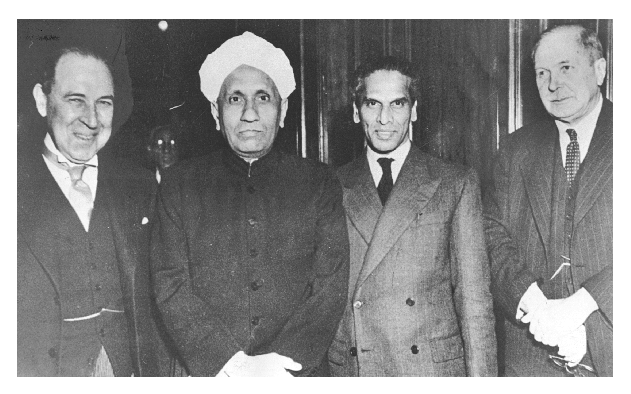
\includegraphics{eps/5.eps}
\end{center}
\vskip -.4cm
{\fontsize{10pt}{11pt}\selectfont{\em Sir John Anderson, C.V. Raman, V.K. Krishna Menon and Sir Charles \hbox{Darwin} at a reception in honour of Raman by the High Commissioner in \hbox{London}, May 11, 1948.} (Photo courtesy : The Hindu.)}\relax
\end{figure}

\begin{figure}[H]
\begin{center}
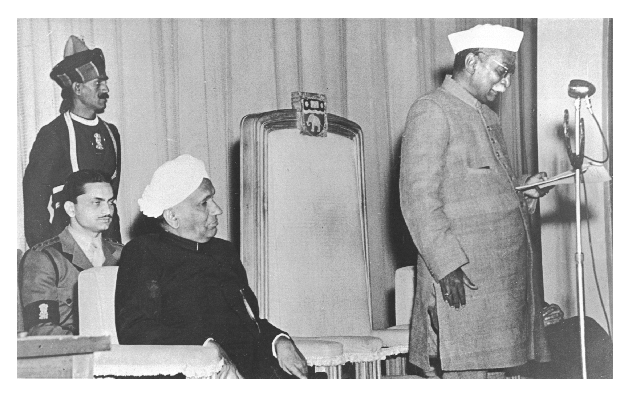
\includegraphics{eps/6.eps}
\end{center}
\vskip -.4cm
{\fontsize{10pt}{11pt}\selectfont{\em President Rajendra Prasad inaugurates the Seventeenth Annual Meeting of the Indian Academy of Sciences on December 27, 1951 in Delhi. Raman is seated on the left.} (Photo courtesy : The Hindu.)}\relax
\end{figure}

\begin{figure}[H]
\begin{center}
\includegraphics[scale=1.05]{eps/8.eps}
\end{center}
\vskip -.4cm
{\fontsize{10pt}{11pt}\selectfont{\em Raman in the company of Nobel Prize men at the conference in Lindau in 1956. Wolfgang Pauli singing in a jovial mood. Max Born, wearing a dotted tie, is seen on the left, first in the second row.} (Photo courtesy : The Hindu.)}\relax
\end{figure}
